%\chapter{Construcción de supercondensadores}
Un supercondensadores es armado simplemente haciendo un sándwich electrodo-separador-electrodo, el electrodo es una lámina de material, de aspecto similar al papel, el sándwich es introduce en la celda de prueba de la figura \ref{fig:celda_de_pruebas_SC}). 

\section{Celda de pruebas de supercondensador}
Se diseña una celda para realizar las pruebas de supercondensadores con los materiales sintetizados. La celda (ver figura \ref{fig:celda_de_pruebas_SC}) consta de dos colectores de corriente de acero inoxidable, entre los que se ubica el condensador como tal. Los colectores de corriente tienen sellos que impiden la fuga del electrolíto o la evaporación del agua en él, permitiendo una operación estable en el tiempo. Los colectores de corriente se apoyan en bloques de acero que cierran la celda con pernos y permitan conectar los terminales del potenciómetro a la celda de pruebas.

\begin{figure}[h!]
	\centering
	\fbox{
		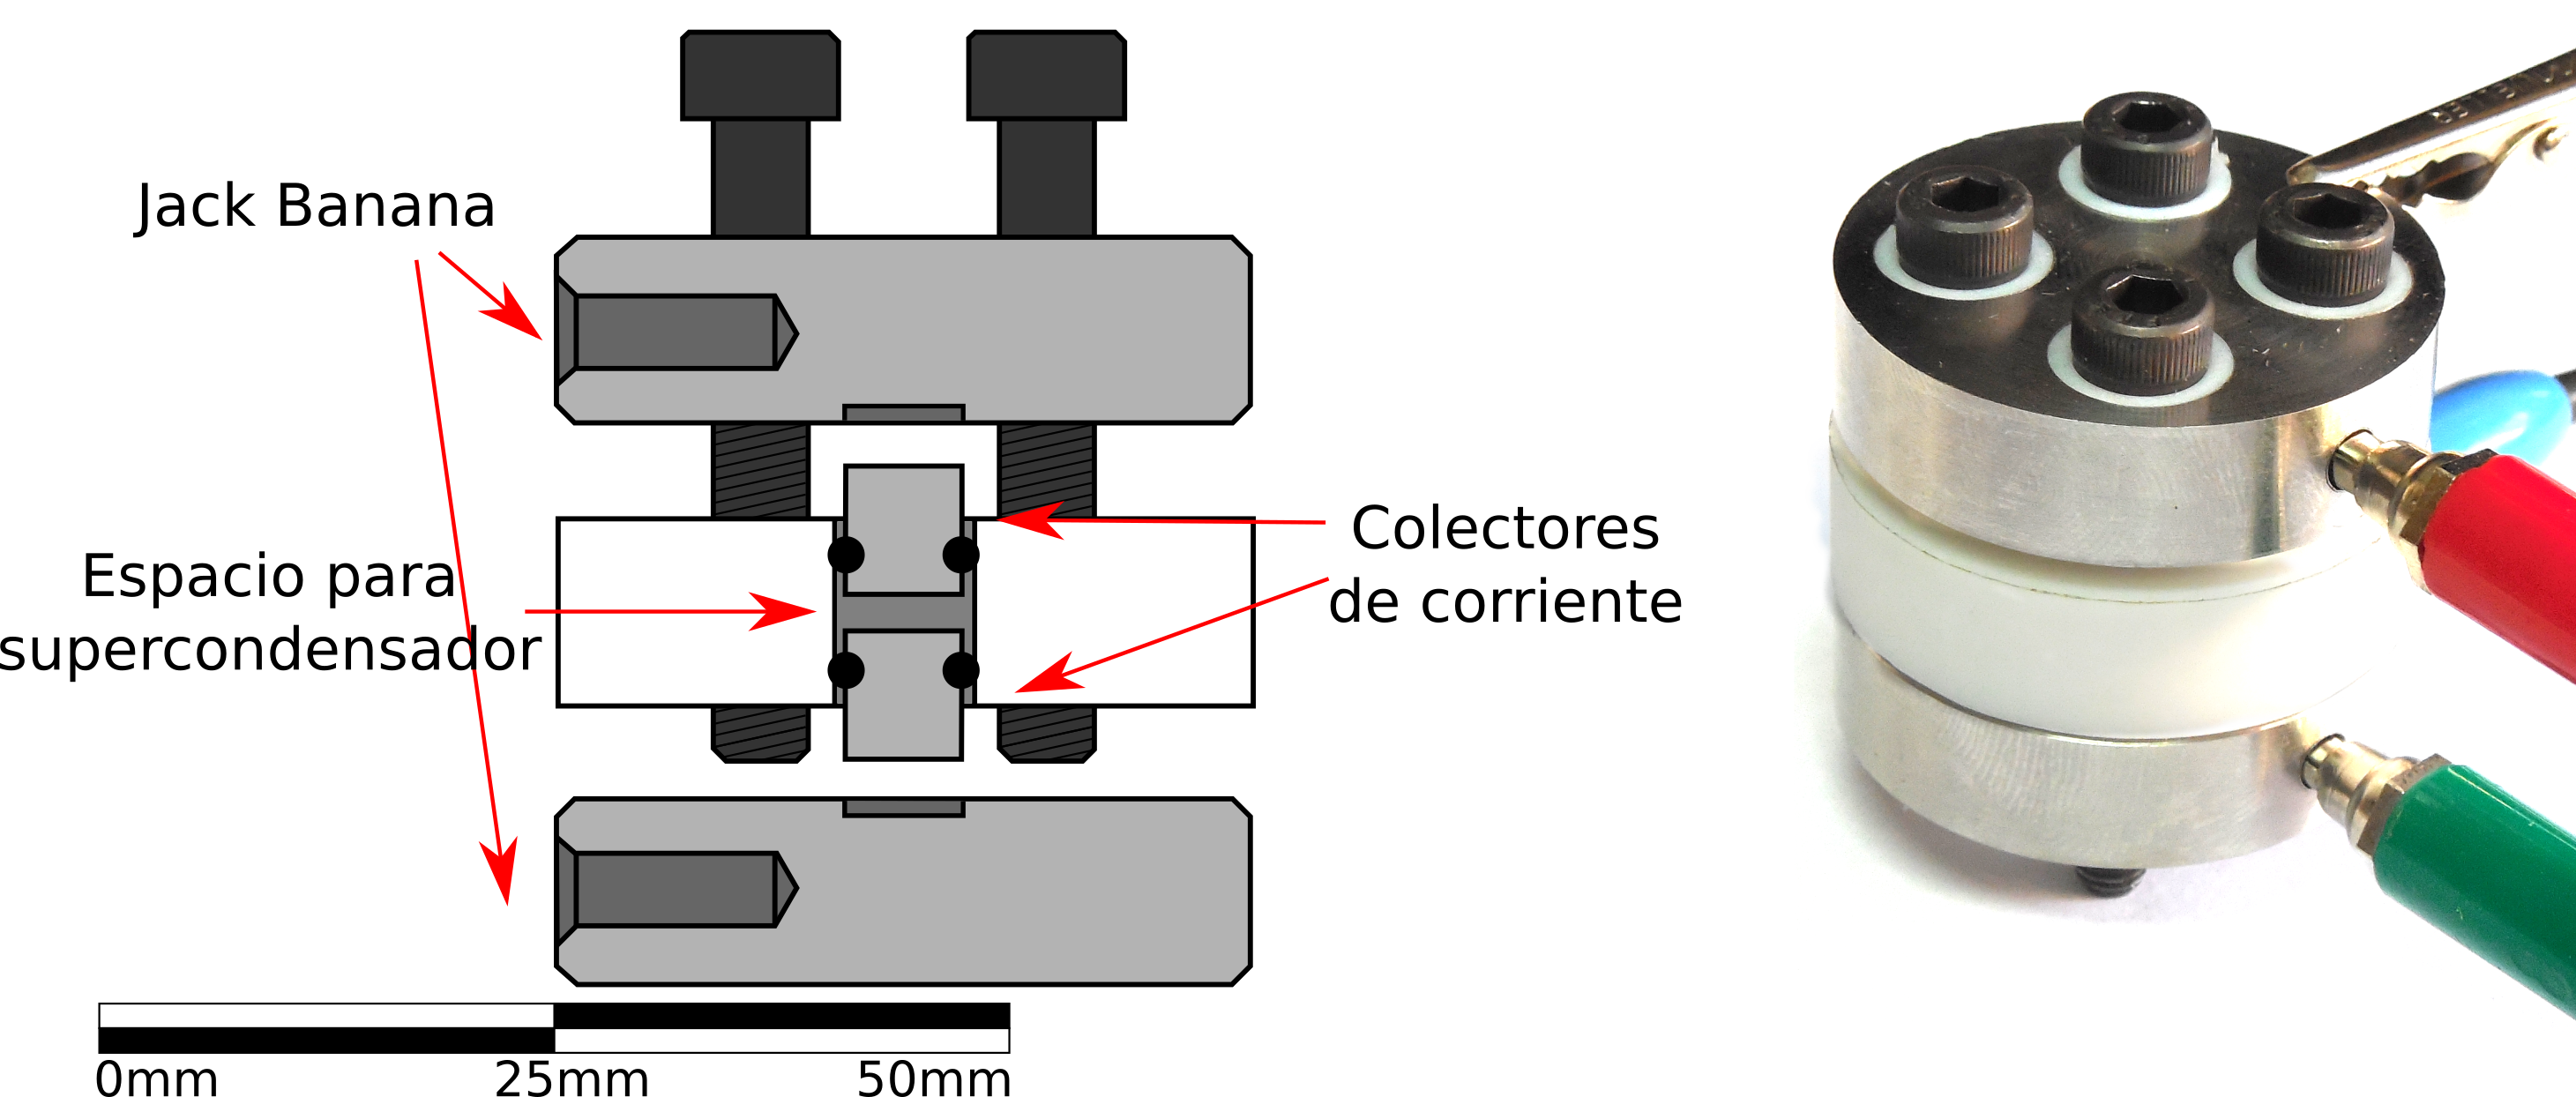
\includegraphics[width=0.8\textwidth]{cell3.png}
		}
	\caption{Derecha: Vista longitudinal de la celda de pruebas, mostrando los componentes más importantes. Izquierda: Fotografía de la celda armada y conectada al potenciostato }
	\label{fig:celda_de_pruebas_SC}
\end{figure}

\section{Construcción de electrodos y preparación de electrolítos}
Los electrodos de rGO son fabricados mediante filtración por vació. En la filtración por vacío, se dispersa el rGO en agua, la que se filtra por un filtro de celulosa en un embudo Büchner conectado a un kitasato y una bomba de vació, el filtro con el material atrapado se deja secar a temperatura ambiente formando una lámina, la que es desprendida con facilidad del filtro de celulosa y luego recortada al tamaño apropiado para la celda de pruebas.

\section{Resultados}
Los supercondensadores son sometidos a pruebas electroquímicas para estudiar su desempeño, estás pruebas incluyen: voltametría cíclica (CV), ciclos de carga y descarga a corriente constante, espectroscopía de impedancia electroquímica (EIS). Todas las mediciones electroquímicas son hechas con un potenciostato/galvanostato (Interface 5000E, Gamry).
